\newcommand{\codeRef}[2][]{\hyperref[section:#2]{\mintinline{java}!#2#1!}}
\chapter{Η εφαρμογή (\appname{})}
\section{Ρυθμίσεις router}
\begin{figure}[htb]
\centering
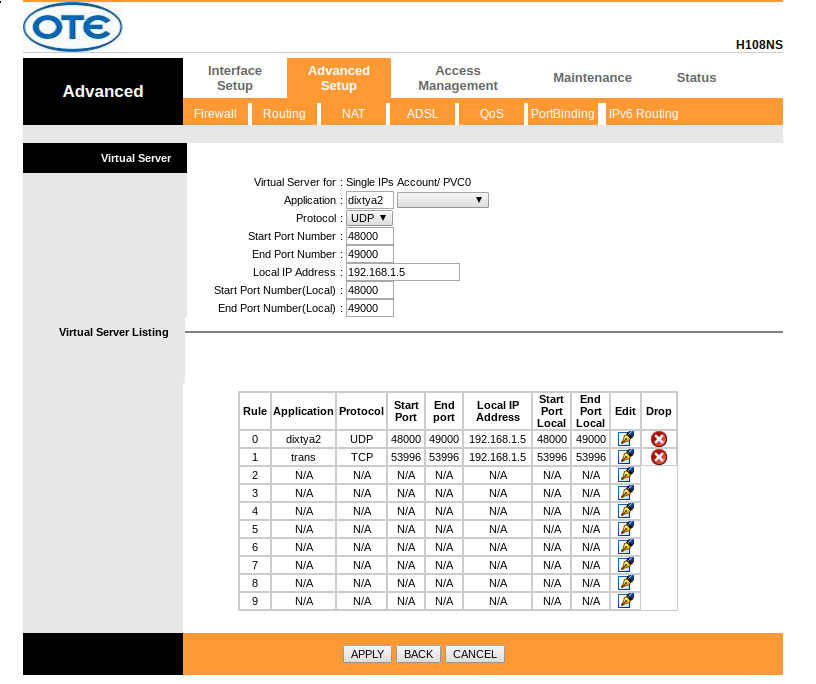
\includegraphics[width=\linewidth]{images/router}
\caption{Ρυθμίσεις router}
\label{fig:router}
\end{figure}
Για την σωστή λειτουργία της εφαρμογής \appname{} χρειάστηκε η αλλαγή ρυθμίσεων του router.
Ακολουθήθηκαν τα εξής βήματα:
\begin{enumerate}
\item Επίσκεψη της σελίδας ρυθμίσεων του router \url{http://192.168.1.1}.
Πρόκειται για μία συσκευή ZTE H108NS, Firmware Version: \texttt{H108NSV1.1.7u\_ZRD\_GR2\_A68}.
\item Εισαγωγή του κωδικού διαχειριστή.
\item Περιήγηση στη σελίδα: \texttt{Advanced Setup > NAT > Virtual Server}.
\item Δημιουργία νέου κανόνα με τις κατάλληλες ρυθμίσεις.
Για τον έλεγχο της ip του μηχανήματος όπου εκτελείται η εφαρμογή εκτελέσαμε:
\begin{code}
\begin{minted}{bash}
$ ifconfig enp2s0
enp2s0: flags=4163<UP,BROADCAST,RUNNING,MULTICAST>  mtu 1500
        inet 192.168.1.5  netmask 255.255.255.0  broadcast 192.168.1.255
        inet6 2a02:587:1808:bb00:5726:d95c:595b:5eae  prefixlen 64  scopeid 0x0<global>
        inet6 fe80::da4c:b00b:629f:ea30  prefixlen 64  scopeid 0x20<link>
        ether 08:60:6e:c7:db:b8  txqueuelen 1000  (Ethernet)
        RX packets 116646  bytes 97594158 (93.0 MiB)
        RX errors 0  dropped 14  overruns 0  frame 0
        TX packets 102421  bytes 56928201 (54.2 MiB)
        TX errors 0  dropped 1 overruns 0  carrier 0  collisions 0
\end{minted}
\caption{Η IP στο τοπικό μηχάνημα}
\end{code}
\begin{code}
\begin{minted}{bash}
$ uname -srmo
Linux 4.4.5-1-ARCH x86_64 GNU/Linux
\end{minted}
\caption{Το λειτουργικό σύστημα του τοπικού μηχανήματος}
\end{code}
Η ρύθμιση φαίνεται στο \imageref{router}.
\end{enumerate}

\section{Script \scriptname{}}\label{section:script}
Για την γρήγορη εξαγωγή των κωδικών από το site \url{http://ithaki.eng.auth.gr/netlab/index.html} γράφτηκε ένα script σε
\href{https://www.python.org/}{python3}
όπου πραγματοποιεί τη σύνδεση (login) με το site με τα σχετικά credentials και εξάγει σε ένα αρχείο τους κωδικούς σε μορφή
\href{https://en.wikipedia.org/wiki/JSON}{json} ώστε να μπορούν εύκολα να διαβαστούν οι τελευταίοι κωδικοί αυτόματα από την εφαρμογή \appname{}.
Χρησιμοποιήθηκαν οι εξωτερικές βιβλιοθήκες:
\begin{itemize}
\item \href{http://docs.python-requests.org/en/master/}{requests} για την πραγματοποίηση της συνεδρίας, και το downloading των σχετικών σελίδων.
\item \href{http://www.crummy.com/software/BeautifulSoup/}{BeautifulSoup} για το parsing των \texttt{.html} αρχείων για την εξαγωγή των κωδικών.
\end{itemize}

Καθώς δεν είναι δυνατό το ανέβασμα επιπλέον αρχείου με το όνομα \scriptname{} ο κώδικας παρατίθεται εδώ:
\begin{code}
\inputminted[frame=single, breaklines=true, linenos=true, python3=true]{python}{../extract-codes.py}
\caption{Το script \scriptname{}}
\label{listing:extract-codes}
\end{code}

\section{Χρήση βιβλιοθηκών \& imports}
\begin{code}
\begin{minted}{java}
import com.google.gson.Gson;
import com.google.gson.JsonObject;
import com.google.gson.stream.JsonReader;

import javax.sound.sampled.AudioFormat;
import javax.sound.sampled.AudioSystem;
import javax.sound.sampled.LineUnavailableException;
import javax.sound.sampled.SourceDataLine;
import java.io.*;
import java.net.*;
import java.nio.ByteBuffer;
import java.nio.ByteOrder;
import java.util.Arrays;
import java.util.logging.ConsoleHandler;
import java.util.logging.Handler;
import java.util.logging.Level;
import java.util.logging.Logger;

import static javax.xml.bind.DatatypeConverter.printHexBinary;
\end{minted}
\caption{Imports στο \appname}
\end{code}

Χρησιμοποιήθηκαν οι εξής βιβλιοθήκες:
\begin{itemize}
\item
\href{https://github.com/google/gson}{\mintinline{java}!com.google.gson.Gson!}:
\begin{displayquote}
Gson is a Java library that can be used to convert Java Objects into their JSON representation. It can also be used to convert a JSON string to an equivalent Java object.
\end{displayquote}
Βιβλιοθήκη της google, για την ανάγνωση και parsing αρχείων τύπου \texttt{JSON}.
Το σχετικό dependency στο maven είναι:
\begin{minted}{xml}
<dependencies>
    <dependency>
        <groupId>com.google.code.gson</groupId>
        <artifactId>gson</artifactId>
        <version>2.6.2</version>
    </dependency>
</dependencies>
\end{minted}
Χρησιμοποιείται αποκλειστικά στη μέθοδο \codeRef{initVariables}.

\item
\href{https://docs.oracle.com/javase/8/docs/api/javax/sound/sampled/package-summary.html}{\mintinline{java}!javax.sound.sampled!}:
\begin{displayquote}
Provides interfaces and classes for capture, processing, and playback of sampled audio data.
\end{displayquote}
Για την αναπαραγωγή ήχου που λαμβάνεται σε μορφή \mintinline{java}!byte[]! (array).
Χρησιμοποιείται στην μέθοδο \codeRef{playMusic}.

\item
\href{https://docs.oracle.com/javase/8/docs/api/java/io/package-summary.html}{\mintinline{java}!java.io.*!}:
\begin{displayquote}
Provides for system input and output through data streams, serialization and the file system.
\end{displayquote}
Χρησιμοποιείται για την διαχείριση αρχείων. Κυρίως για την αποθήκευση των αποτελεσμάτων.

\item
\href{https://docs.oracle.com/javase/8/docs/api/java/net/package-summary.html}{\mintinline{java}!java.net.*!}:
\begin{displayquote}
Provides the classes for implementing networking applications.
\end{displayquote}
Περιλαμβάνει κλάσεις διαχείρισης δικτυακών πόρων.
Παρέχει τις πολύ βασικές κλάσεις για την εφαρμογή μας:
\mintinline{java}!DatagramPacket! και \mintinline{java}!DatagramSocket!.
Χρησιμοποιείται σε όλες τις μεθόδους που έχουν σχέση με τον server της Ιθάκης.

\item
\href{https://docs.oracle.com/javase/8/docs/api/java/nio/package-summary.html}{\mintinline{java}!java.nio!}:
\begin{displayquote}
Defines buffers, which are containers for data, and provides an overview of the other NIO packages.
\end{displayquote}
Χρησιμοποιείται για διάφορες λειτουργικότητες σχετικές με buffers.

\item
\href{https://docs.oracle.com/javase/8/docs/api/java/util/package-summary.html}{\mintinline{java}!java.util!}:
\begin{displayquote}
Contains the collections framework, legacy collection classes, event model, date and time facilities, internationalization, and miscellaneous utility classes (a string tokenizer, a random-number generator, and a bit array).
\end{displayquote}
\sloppy Χρησιμοποιούνται διάφορες βασικές λειτουργίες όπως:
\mintinline{java}!java.util.logging! και \mintinline{java}!java.util.Arrays!.
\end{itemize}

\section{Η \mintinline{java}!class userApplication!}
\begin{code}
\begin{minted}{java}
/**
 * Main application for the assignment.
 */
class userApplication {
    private final static Level loggerLevel = Level.ALL;
    private final static Logger logger = Logger.getLogger(userApplication.class.getName());

    static {
        // http://stackoverflow.com/questions/6315699/why-are-the-level-fine-logging-messages-not-showing
        final Handler consoleHandler = new ConsoleHandler();
        consoleHandler.setLevel(loggerLevel);
        logger.setUseParentHandlers(false);
        logger.addHandler(consoleHandler);
        logger.setLevel(loggerLevel);
    }

    public static void main(final String[] args) throws IOException, LineUnavailableException {
        final MainInstance app = new MainInstance();
        app.run(args);
    }

    private static class MainInstance {...}
}
\end{minted}
\caption{Η εξωτερική κλάση \mintinline{java}!userApplication!}
\end{code}
Αποτελεί την εξωτερική κλάση που υλοποιεί την εφαρμογή.
Ρόλος της είναι:
\begin{itemize}
\item Η αρχικοποίηση ενός αντικειμένου \mintinline{java}!Logger logger! που βοηθάει στο debugging και την εκτύπωση μηνυμάτων.
\item Η κλήση της \mintinline{java}!public static void main()! που αρχικοποιεί ένα αντικείμενο της βασικής κλάσης \codeRef{MainInstance}.
\end{itemize}
